\documentclass{article}

\usepackage[a4paper, total={6in, 8in}]{geometry}
\usepackage[breakable]{tcolorbox}
\usepackage{parskip} % Stop auto-indenting (to mimic markdown behaviour)
\usepackage{graphicx} % Required for inserting images
\usepackage{physics}
\usepackage{amsthm}
\usepackage{amssymb}
\usepackage{mathtools}
\usepackage{amsmath}
\usepackage{enumerate}

\title{PC3233 Assignment 3}
\author{Hor Zhu Ming (A0236535A)}
\date{Feb 2024}

\begin{document}

\maketitle

\section{Stern-Gerlach Experiment}

From question, we have the following information:
\begin{equation}
  \begin{cases}
    & \dv{B}{z} = 10^3 \text{ T/m} \\
    & l_1 = 4 \times 10^{-2} \text{ m} \\
    & l_2 = 10 \times 10^{-2} \text{ m} \\
    & d = 2 \times 10^{-3} \text{ m} \\
    & v = 500 \text{ m/s} \\
    & M = 1.79 \times 10^{-25} \text{ kg} \\
  \end{cases}
\end{equation}

From lecture, we know that potential energy of a magnetic dipole in a magnetic field is given by:

\begin{equation}
  E_{\text{pot}} = - \vec{\mu} \cdot \vec{B}
\end{equation}

And the Lorentz force is given by:

\begin{align*}
  \vec{F} 
  &= - \vec{\nabla} E_{\text{pot}} \\
  & = \vec{\nabla} (\vec{\mu} \cdot \vec{B}) \\
  & = \mu_z \dv{B}{z} \hat{z} \\
  & = \mu_z 10^3 \hat{z}
\end{align*}

Therefore, using Newton's second law, we can find the acceleration of the particle:

\begin{align*}
  \vec{F} 
  &= M \vec{a} \\
  \mu_z 10^3 &= M a \\
  a &= \frac{\mu_z 10^3}{M}
\end{align*}

Since the acceleration is constant and perpendicular to the initial velocity, $v$, we can 
use the following kinematic equation to find the time taken for the particle to travel from distance of $l_1$ and $l_2$ in the x-direction, $t_1$ and $t_2$ respectively:

\begin{align*}
  t_1 &= \frac{l_1}{v} = \frac{4 \times 10^{-2}}{500} = 8 \times 10^{-5} \text{ s} \\
  t_2 &= \frac{l_2}{v} = \frac{10 \times 10^{-2}}{500} = 2 \times 10^{-4} \text{ s}
\end{align*}

Then, with the initial velocity in z-direction of $v_{z_i}$ which is $0 \text{ m/s}$,
we express the distance travelled in the z-direction as a function of $\mu_z$:

\begin{align*}
  \frac{d}{2} &= s_{y1} + s_{y2} \hspace{2in}s = v_{i}t + \frac{1}{2}a t^2 \\
  \frac{d}{2} &= v_{z_i}t_1 + \frac{1}{2}a t_1^2 + v_{z_f}t_2\\
  \frac{d}{2} &= \frac{1}{2}a t_1^2 + v_{z_f}t_2 \hspace{2in} v_{z_f} = v_{z_i} + at_1 \\
  \frac{d}{2} &= \frac{1}{2}a t_1^2 + (at_1)t_2 \hspace{2in} \text{where } a = \frac{\mu_z 10^3}{M} \\
  d &= \mu_z \frac{10^3}{M} \left(t_1^2 + 2t_1t_2\right) \\
\end{align*}

Rearrange to get $\mu_z$, then substitute the values to get the answer:

\begin{align*}
  \mu_z &= \frac{dM}{10^3 \left(t_1^2 + 2t_1t_2\right)} \\
  &= \frac{2 \times 10^{-3} \times 1.79 \times 10^{-25}}{10^3 \left((8 \times 10^{-5})^2 + 2 (8\times10^{-5})(2 \times 10^{-4})\right)} \\
  &= 9.323 \times -24 \text{ A m}^2
\end{align*}

For second part, why doesn't the nuclear spin affect the experiemnt?

The deflection depends on the strength of magnetic dipole moment, $\mu$.

For electron, the magnetic dipole moment is given by:

\begin{equation}
  \mu_e \approx 2 \mu_B = \frac{e\hbar}{2m_e} \hspace{2in} \text{where } \mu_B = \frac{e\hbar}{2m_e}
\end{equation}

For nuclear, the magnetic dipole moment is given by:

\begin{equation}
  \mu_{\text{nuclear}} \approx \mu_N = \frac{e\hbar}{2m_p} \hspace{2in} \text{where } \mu_N = \frac{e\hbar}{2m_p}
\end{equation}

Then,

\begin{equation}
  \frac{\mu_N}{\mu_e} = \frac{m_e}{m_p} \approx \frac{1}{1836} \ll 1
\end{equation}

So the deflection of the proton is much smaller than the electron, and hence the 
nuclear spin does not affect the experiment.

\section{Coupling of Angular Momentum}

\subsection{Part a}

For uncoupled bases, $J_1^2$, $J_2^2$, $J_{z1}$ and $J_{z2}$ are the commuting observable which 
can be simultaneously diagonalized with basis specified by the quantum numbers $j_1$, $j_2$, $m_1$ 
and $m_2$ respectively. Hence,  $j_1$, $j_2$, $m_1$ and $m_2$ are good quantum numbers.

Similarly, for coupled bases, $J^2$, $J_z$, $J_1^2$, $J_2^2$ are the commuting observable which can be
simultaneously diagonalized with basis specified by the quantum numbers $j$, $m$, $j_1$ and $j_2$
respectively. Hence, $j$, $m$, $j_1$ and $j_2$ are good quantum numbers.

\subsection{Part b}

Prove the commutation relation:

\begin{equation}
  \commutator{J^2}{J_i^2} = 0
\end{equation}

We know that $J^2$ is given by $J^2 = J_1^2 + J_2^2 + 2J_1 \cdot J_2$. Then, we can write the commutator as:

\begin{align*}
  \commutator{J^2}{ J_i^2} &= \commutator{J_1^2 + J_2^2 + 2J_1 \cdot J_2}{J_i^2} \\
  &= \commutator{J_1^2}{J_i^2} + \commutator{J_2^2}{J_i^2} + \commutator{2J_1 \cdot J_2}{J_i^2} \\
\end{align*}

Both $\commutator{J_1^2}{J_i^2}$ and $\commutator{J_2^2}{J_i^2}$ are zero 
either because $J_i^2$ is acting on a non-$i$ space $J^2$ operator or 
$J_i^2$ is acting on the itself. Hence,
\begin{align*}
  \commutator{J_1^2}{J_i^2} + \commutator{J_2^2}{J_i^2} + \commutator{2J_1 \cdot J_2}{J_i^2} &= 0 + 0 + 2[J_1 \cdot J_2, J_i^2] \\
  &= 2([J_1, J_i^2]J_2 + J_1[J_2, J_i^2]) \\
\end{align*}

Similar argument to above can be made for the commutator $[J_1, J_i^2]$ and $[J_2, J_i^2]$ either
because $J_i^2$ is acting on a non-$i$ space $J$ operator or $\commutator{J_i^2}{J_i} = \commutator{J_i}{J_i}J_i 
+ J_i\commutator{J_i}{J_i} = 0$. Hence,

\begin{align*}
  2([J_1, J_i^2]J_2 + J_1[J_2, J_i^2]) &= 2(0 + 0) \\
  &= 0
\end{align*}

Therefore, $\commutator{J^2}{J_i^2} = 0$.

\subsection{Part c}

Given two angular momenta with given quantum numbers $j_1$ and $j_2$, the possible quantum numbers
for $J^2$ is:

\begin{equation}
j \in \{\abs{j_1 - j_2}, \abs{j_1 - j_2} + 1, \ldots,  j_1 + j_2\}
\end{equation}

And the possible quantum numbers for $J_z$ is:

\begin{equation}
  m \in \{-j, -j+1, \ldots, j-1, j\}
\end{equation}

Below is the illustration for $J^2$ when $j_1 = 1$ and $j_2 = 1$:

\begin{figure}[h!]
  \centering
  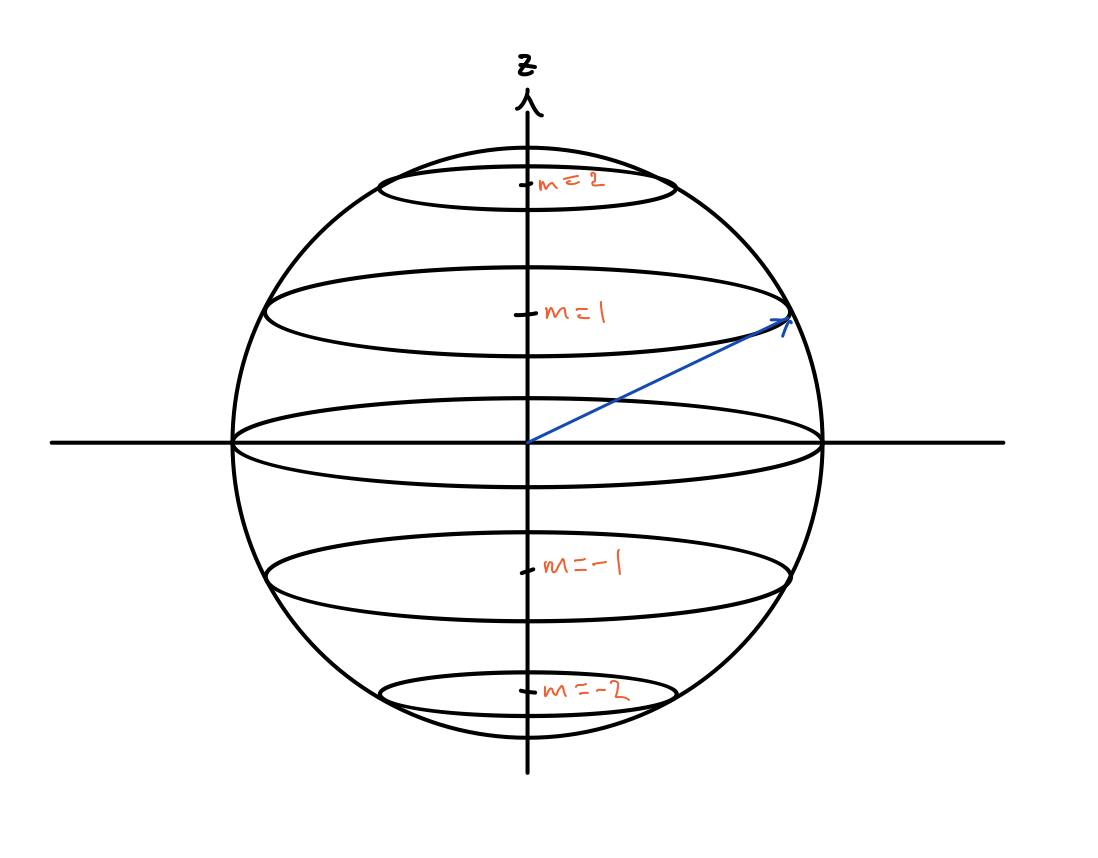
\includegraphics[width=5in]{../image/AngularMomentumVectorModel.jpg}
  \caption{illustration for $J^2$ when $j_1 = 1$ and $j_2 = 1$}
\end{figure}


\subsection{Part d}

Given the general basis transformation from uncoupled to coupled basis:

\begin{equation}
  \ket{j_1, j_2, j, m} 
  = \sum_{j_1^{'}, j_2^{'}}
  \sum_{m_1, m_2} 
  \ket*{j_1^{'}, j_2^{'}, m_1, m_2}
  \bra*{j_1^{'}, j_2^{'}, m_1, m_2} 
  \ket{j_1, j_2, j, m}
\end{equation}

We want to prove that the Clebsch-Gordan coefficients 
$\bra*{j_1^{'}, j_2^{'}, m_1, m_2} \ket{j_1, j_2, j, m}$ is not zero
if and only if:
\begin{enumerate}[(i)]
  \item $m = m_1 + m_2$
  \item $j_1^{'} = j_1$ and $j_2^{'} = j_2$
\end{enumerate}

To prove (i), we act the null operator $J_z - J_z^{(1)} - J_z^{(2)} = 0$ in between
$\bra*{j_1^{'}, j_2^{'}, m_1, m_2} \ket{j_1, j_2, j, m}$:

\begin{equation}
  \bra*{j_1^{'}, j_2^{'}, m_1, m_2} (J_z - J_z^{(1)} - J_z^{(2)}) \ket{j_1, j_2, j, m} = 0 
\end{equation}

Then, we can evaluate the above equation to get:

\begin{equation}
  (m - m_1 - m_2) \bra*{j_1^{'}, j_2^{'}, m_1, m_2} \ket{j_1, j_2, j, m} = 0
\end{equation}

\textit{Proof. i.}

\textbf{Case 1: $m \neq m_1 + m_2$} \\
If $m \neq m_1 + m_2 \implies m - m_1 - m_2 \neq 0$, then the above equation is 
satisfied if and only if the Clebsch-Gordan coefficient, $\bra*{j_1^{'}, j_2^{'}, m_1, m_2} \ket{j_1, j_2, j, m} = 0$

\textbf{Case 2: $m = m_1 + m_2$} \\
If $m = m_1 + m_2 \implies m - m_1 - m_2 = 0$, then the Clebsch-Gordan coefficient, $\bra*{j_1^{'}, j_2^{'}, m_1, m_2} \ket{j_1, j_2, j, m}$ 
can be any arbitary value.

Therefore, we have proved (i).

With a similar idea, we can prove (ii) by acting the null operator $J^{2 (1)} - J^{2(1)} = 0$ in between
$\bra*{j_1^{'}, j_2^{'}, m_1, m_2} \ket{j_1, j_2, j, m}$:

\begin{equation}
  \bra*{j_1^{'}, j_2^{'}, m_1, m_2} (J^{2(1)} - J^{2(1)}) \ket{j_1, j_2, j, m} = 0
\end{equation}

Then, we can evaluate the above equation to get:

\begin{equation}
  (\hbar j_1^{'}(j_1^{'}+1) - \hbar j_1(j_1+1)) \bra*{j_1^{'}, j_2^{'}, m_1, m_2} \ket{j_1, j_2, j, m} = 0
\end{equation}

\textit{Proof. ii.a}

\textbf{Case 1: $j_1^{'} \neq j_1$} \\
Then $\hbar j_1^{'}(j_1^{'}+1) - \hbar j_1(j_1+1) \neq 0$, then the above equation is
satisfied if and only if the Clebsch-Gordan coefficient, $\bra*{j_1^{'}, j_2^{'}, m_1, m_2} \ket{j_1, j_2, j, m} = 0$

\textbf{Case 2: $j_1^{'} = j_1$} \\
Then $\hbar j_1^{'}(j_1^{'}+1) - \hbar j_1(j_1+1) = 0$, then the Clebsch-Gordan coefficient, $\bra*{j_1^{'}, j_2^{'}, m_1, m_2} \ket{j_1, j_2, j, m}$
can be any arbitary value.

Without loss of generality, we can prove for $j_2^{'} = j_2$ as well by null operator $J^{2 (1)} - J^{2(1)} = 0$ in between
$\bra*{j_1^{'}, j_2^{'}, m_1, m_2} \ket{j_1, j_2, j, m}$. (\textit{Proof. ii.b})

To combine the two conclusions from (\textit{ii.a}) and (\textit{ii.b}), we need to consider four cases:
\begin{enumerate}
  \item $j_1^{'} \neq j_1$ and $j_2^{'} \neq j_2$, then the Clebsch-Gordan coefficient, $\bra*{j_1^{'}, j_2^{'}, m_1, m_2} \ket{j_1, j_2, j, m} = 0$
  \item $j_1^{'} = j_1$ and $j_2^{'} \neq j_2$, then the Clebsch-Gordan coefficient, $\bra*{j_1^{'}, j_2^{'}, m_1, m_2} \ket{j_1, j_2, j, m}$ = 0.
  \item $j_1^{'} \neq j_1$ and $j_2^{'} = j_2$, then the Clebsch-Gordan coefficient, $\bra*{j_1^{'}, j_2^{'}, m_1, m_2} \ket{j_1, j_2, j, m}$ = 0.
  \item $j_1^{'} = j_1$ and $j_2^{'} = j_2$, then the Clebsch-Gordan coefficient, $\bra*{j_1^{'}, j_2^{'}, m_1, m_2} \ket{j_1, j_2, j, m}$ can be any arbitary value.
\end{enumerate}

Hence, we have proved (ii).

\end{document}
